\documentclass[tikz,border=6pt]{standalone}
\usepackage{pgfplots}
\pgfplotsset{compat=1.18}
\definecolor{complexorange}{RGB}{234,88,12}

\begin{document}
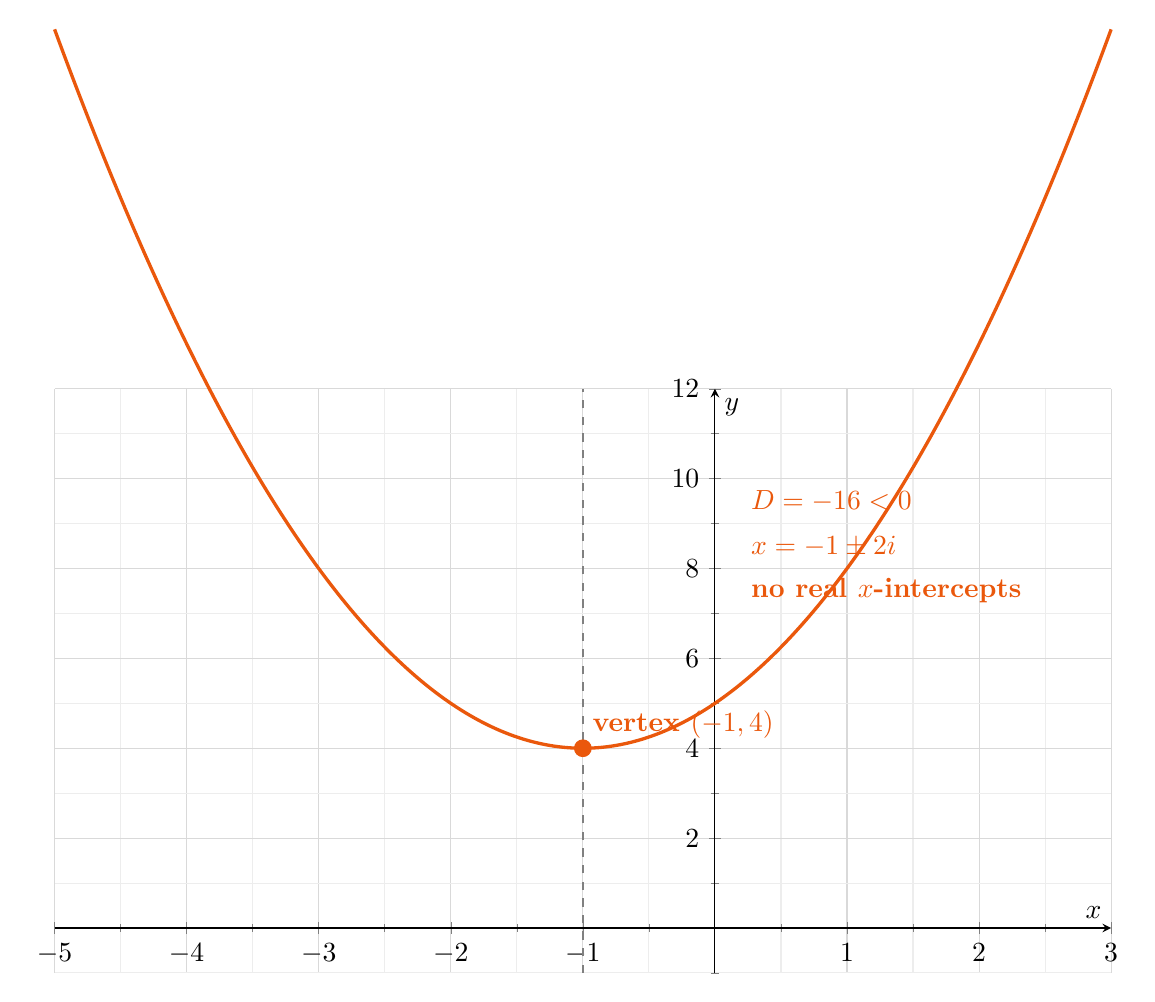
\begin{tikzpicture}
\begin{axis}[
  width=15cm,
  height=9cm,
  xmin=-5,
  xmax=3,
  ymin=-1,
  ymax=12,
  axis lines=middle,
  xlabel={$x$},
  ylabel={$y$},
  grid=both,
  minor tick num=1,
  major grid style={draw=gray!30},
  minor grid style={draw=gray!14},
  samples=240,
  clip=false
]

\addplot[complexorange,very thick,domain=-5:3]{x^2+2*x+5};
\addplot[gray,dashed,thick] coordinates {(-1,-1) (-1,12)};
\addplot[complexorange,only marks,mark=*,mark size=3pt]
  coordinates {(-1,4)};

\node[complexorange,font=\bfseries,anchor=south west]
  at (axis cs:-1,4) {vertex $(-1,4)$};

\node[complexorange,font=\bfseries,anchor=west]
  at (axis cs:0.2,9.5) {$D=-16<0$};

\node[complexorange,font=\bfseries,anchor=west]
  at (axis cs:0.2,8.5) {$x=-1\pm2i$};

\node[complexorange,font=\bfseries,anchor=west]
  at (axis cs:0.2,7.5) {no real $x$-intercepts};

\end{axis}
\end{tikzpicture}
\end{document}
